\section{Introdução}
\subsection{Interferometria Atômica e Gravimetria}

Interferômetros atômicos são ferramentas versáteis que permitem a medição de acelerações e rotações com precisão absoluta e alta estabilidade \cite{geiger2020highaccuracy}. Eles desempenham um papel crítico na física fundamental ao conduzir testes quânticos do princípio da equivalência de Einstein \cite{asenbaum2020atom}, medir constantes fundamentais \cite{rosi2014precision}\cite{morel2020determination}, estabelecer limites para modelos de Energia Escura \cite{elder2016chameleon}, e detectar forças de Casimir. Com os avanços na maturidade técnica e na redução de tamanho, esses dispositivos são agora utilizados para gravimetria absoluta terrestre \cite{menoret2018gravity} e estão se tornando essenciais para estudos do sistema climático. Os primeiros experimentos de interferometria atômica conduzidos em foguetes de sondagem \cite{becker2018space}, na Estação Espacial Internacional \cite{aveline2020observation}, e o desenvolvimento do pathfinder de interferometria atômica baseada em satélite CARIOQA \cite{lévèque2022carioqa} para pesquisas do sistema climático destacam o potencial e a importância deste campo. Além disso, existem propostas para usar interferometria atômica para detectar ondas gravitacionais \cite{badurina2022prospective}.

O interferômetro consiste, em sua configuração mais difundida, de uma sequência de três transições Raman $\pi/2$ - $\pi$ - $\pi/2$ contrapropagantes, cada uma separada por um tempo de evolução livre T. Os três pulsos são realizados com as mesmas potências de laser, mas com diferentes durações, respectivamente, de $\tau/2$ - $\tau$ - $\tau/2$. O primeiro pulso divide a função de onda atômica em uma superposição coerente de dois pacotes de ondas parciais, em diferentes estados hiperfinos, e, mais importante, em diferentes estados de momento, uma vez que o pacote de onda "difratado" recebe dos lasers Raman contrapropagantes uma transferência de momento correspondente a duas vezes o momento de um fóton. Durante o primeiro intervalo T de evolução livre, os dois braços do interferômetro então se separam. O segundo pulso atua em ambos os braços do interferômetro, trocando os níveis hiperfinos dos dois pacotes de ondas e seus momentos. Como resultado do pulso $\pi$, os dois pacotes de ondas se aproximam e se sobrepõem após um segundo intervalo de tempo T. Finalmente, o último pulso $\pi/2$ recombina os dois braços do interferômetro para que interfiram \cite{cheinet2006conception}.

O processo do interferômetro é muito semelhante a um experimento de Ramsey, onde a fase de um qubit/sistema de dois níveis é deixada para evoluir livremente por um período entre dois pulsos $\pi/2$. O pulso $\pi$ no meio serve para fazer as ondas de matéria convergirem, em vez de divergirem como antes do pulso, para que a interferência possa ocorrer entre os dois braços. Assim, o pulso $\pi$ atua de maneira muito semelhante aos espelhos em um interferômetro de luz de Mach-Zehnder, onde também os pulsos $\pi/2$ seriam os divisores de feixe (ver figura \ref{fig:interf}).

\begin{figure}
    \centering
    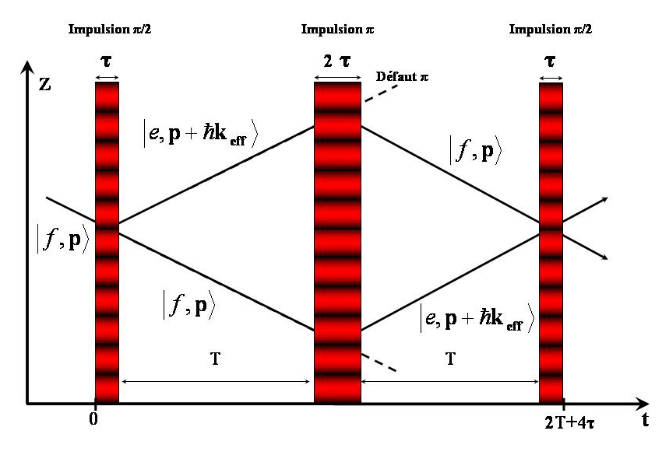
\includegraphics[width=0.7\linewidth]{figures/interferometry.png}
    \caption{Adaptado de \cite{cheinet2006conception}. Esquema da interferometria atômica com pulsos Raman em vermelho.}
    \label{fig:interf}
\end{figure}

Os níveis atômicos podem então ser detectados seletivamente com fluorescência. A probabilidade de detectar o estado hiperfino excitado é dada por:
\begin{equation}
P_e(2T+2\tau)= \frac{1- A\cos(\overrightarrow{g}\cdot \overrightarrow{k}_{\mathrm{eff}}T^2)}{2}
\end{equation}
Onde $\Delta\phi = \overrightarrow{g}\cdot \overrightarrow{k}_{\mathrm{eff}}T^2$ ou número de onda vezes a distância é a fase acumulada da trajetória da onda de matéria, $g$ é a aceleração da gravidade, $k_{\mathrm{eff}}$ é dado pela diferença dos vetores de onda dos dois lasers contrapropagantes (a transferência de momento correspondente é $\hbar \overrightarrow{k}_{\mathrm{eff}}= \hbar(\overrightarrow{k}_1-\overrightarrow{k}_2)$) e $A$ o contraste. A partir dessa relação podemos deduzir $g$ \cite{dos2008gravimetre}.

%\urf{https://metrologie-francaise.lne.fr/sites/default/files/media/document/p33-40-rfm13-pereira-gravimetre-atomes-froids.pdf}

%\url{https://theses.hal.science/tel-00070861}

\subsection{Squeezing}
Na mecânica quântica, o princípio da incerteza de Heisenberg fornece a relação para duas variáveis conjugadas que não comutam. Por exemplo, posição (X) e momento (P):
\begin{equation}
    \Delta X \Delta P \ge \frac{\hbar}{2}
    \label{eq:saymyname}
\end{equation}
Ou também para tempo (t) e energia (E). Um estado coerente, onde há incerteza mínima, satisfaz a condição 
\begin{equation}
    \Delta X = \Delta P = \sqrt{\frac{\hbar}{2}}
\end{equation}
O princípio da incerteza na equação \ref{eq:saymyname} não pode ser violado. Mas podemos escolher um estado para fazer $\Delta X$ ou $\Delta P$ menor que $\sqrt{\hbar/2}$, um estado chamado de estado coerente comprimido ou "squeezed", onde trocamos incerteza em uma variável pela incerteza em sua variável conjugada
%\url{https://arxiv.org/pdf/1011.2978.pdf}
\cite{Ma_2011}.

No nosso caso, as variáveis conjugadas são a estimativa de fase do interferômetro e o número de população/átomos em um estado de saída. Isso seria análogo à fase e ao número de fótons em um interferômetro regular com luz. O objetivo é reduzir a incerteza na estimativa de fase.

\subsection{Delta-Kick Squeezing (DKS)}
A incerteza na estimativa de fase para interferômetros atômicos é limitada inferiormente pelo limite quântico padrão (SQL em inglês), $\Delta \theta_{SQL} = 1/\sqrt{N}$. Onde N é o número não correlacionado de átomos no interferômetro. Ao comprimir a estimativa de fase, essa limitação é superada com o método DKS proposto para melhorar a geração de emaranhamento em interferômetros atômicos de queda livre usando interações átomo-átomo dentro de condensados de Bose-Einstein (BECs).

A ideia principal consiste em focar as ondas de matéria através da aplicação rápida de um potencial de armadilha externo, em analogia com a óptica, onde a armadilha desempenha o papel de uma lente convergente. Passar pelo ponto focal aumenta a densidade da onda de matéria e, assim, a força efetiva das interações partícula-partícula, preparando os átomos em um estado altamente emaranhado e comprimido em spin. Considerando trabalhos anteriores sobre colimação delta-kick, a equipe designou a técnica como delta-kick squeezing (DKS)
%\url{https://arxiv.org/pdf/2103.10896.pdf}
\cite{Corgier_2021}.

\subsection{Transição Raman Estimulada}
Para fazer um interferômetro atômico é necessário criar uma superposição coerente de dois estados quânticos de um átomo e, em seguida, recombinar os pacotes de ondas. Uma transição eletromagnética pode alcançar essa superposição, enquanto transfere o momento do fóton para o segundo estado quântico. Os dois estados então possuem momentos diferentes e o interferômetro será sensível a forças inerciais.

Os dois estados quânticos devem ter uma longa vida útil em relação à duração do experimento. No caso de átomos alcalinos (em nosso experimento, Rb-87), os dois subníveis hiperfinos do estado fundamental podem ser usados \cite{cheinet2006conception}.

No entanto, não excitamos diretamente o átomo entre esses dois níveis. Para isso, seria necessário implementar micro-ondas em nosso experimento, cujos fótons têm um momento muito pequeno e levariam a uma área de interferômetro atômico negligenciável e, assim, a uma pequena sensibilidade. Em vez disso, realizamos uma transição de dois fótons com lasers com um comprimento de onda próximo de 780nm. Ao usar uma transição de dois fótons, esses níveis podem ser acoplados diretamente, como mostrado na figura \ref{fig:levels}.
%Na verdade, combinamos dois lasers que, um, excita do estado fundamental para um estado muito mais alto. E o outro desexcita o átomo para o estado hiperfino. Ambos com um grande desvio do estado intermediário superior, para que não tenhamos qualquer população significativa nem emissões espontâneas desse nível, figura \ref{fig:levels}.

\begin{figure}
    \centering
    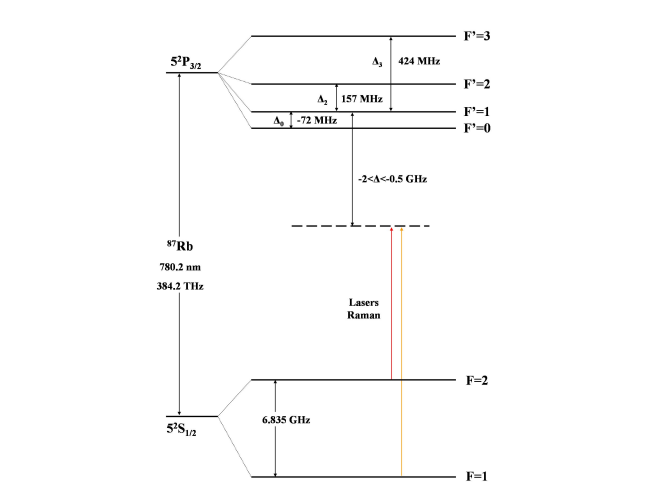
\includegraphics[width=0.8\linewidth]{figures/raman-levels.png}
    \caption{Níveis de $^{87}$Rb com transições de lasers Raman e desacordo $\Delta$. Adaptado de \cite{cheinet2006conception}.}
    \label{fig:levels}
\end{figure}

\subsection{Visão Geral}
Na seção de métodos, explicarei o trabalho realizado no laboratório para melhorar o laser Raman em vários aspectos. Primeiro, a implementação do \gls{TA} para aumentar a potência do laser Raman, depois a trava de offset para evitar a variação do offset geral dos lasers (o que faria a frequência de Rabi e a emissão espontânea variar), depois a trava de estabilização de potência para reduzir as flutuações nas fidelidades dos pulsos e, finalmente, as próprias transições atômicas onde podemos demonstrar o funcionamento dos lasers Raman.

Nos resultados, mostrarei e discutirei os desempenhos e resultados do meu trabalho, incluindo uma realização do gravímetro em si e a medição da gravidade que obtivemos.
